\section[Adaptive systems]{\Glspl{adptSyst}}
%\label{sec:back:adapt-syst}

This section introduces the background to understand \glspl{adptSyst}.
First, we describe the principles and vision of \glspl{adptSyst}.
Before we characterise the information used by an adaptation process, we detail a model-based technique to implement them: \gls{m@rt}.
Finally, we highlight the key concepts used in this thesis and link them to the contributions.

\subsection{Principles and vision}
\begin{figure}
	\centering
	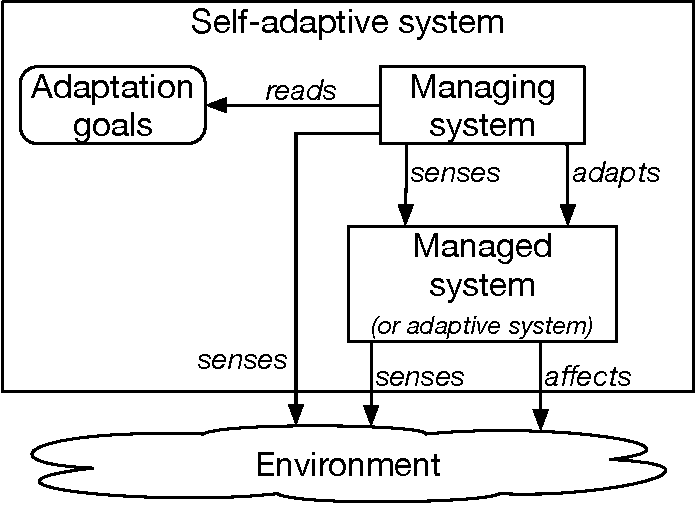
\includegraphics[width=0.5\linewidth]{img/chapt-background/adptSyst/vision}
	\caption{Conceptual vision of \gls{adptSyst} (based on \cite{DBLP:books/sp/19/Weyns19})}
	\label{fig:background:adptSyst:principles}
\end{figure}

%The complexity of nowadays software systems comes with laborious, error-prone, and redundant tasks (installation, configuration, maintenance, \etc) for developers.
%Moreover, software systems can be executed in uncertain and evolving \glspl{env}~\cite{DBLP:conf/dagstuhl/EsfahaniM10}.
%Following the autonomic computing vision pushed by IBM engineers~\cite{computing2006architectural}, Kephart and Chess have established the basis for \glspl{adptSyst}~\cite{DBLP:journals/computer/KephartC03}.

\Glspl{adptSyst} take their origins in the vision paper of Kephart and \linebreak Chess~\cite{DBLP:journals/computer/KephartC03}, which is based on the autonomic computing vision pushed by IBM engineers~\cite{computing2006architectural}.
These systems are recognised by their ability to have their behaviour or structure adapted automatically in response to changes in their \gls{env} or of the systems themselves.
This adaptation helps them to achieve their goals based on high-level objectives~\cite{DBLP:conf/dagstuhl/ChengLGIMABBBCSDFGGGKKKLMMMPSTTWW09}.
If a system performs itself this adaptation mechanism with minimal interference, the literature refers to it as a \gls{sadapt}~\cite{DBLP:conf/dagstuhl/BrunSGGKLMPS09}.\looseness-1

Danny Weyns	identified two principles for \glspl{adptSyst}~\cite{DBLP:books/sp/19/Weyns19}: the internal and the external principles.
The former one is based on the \textquote{discipline split} defined by Andersson \etal ~\cite{DBLP:conf/icse/AnderssonLMW09}: each \gls{adptSyst} can be split into two concerns.
First, the domain concern categorises the part of the system that deals with the purpose for which the system has been built.
Second, the adaptation concern handles the adaptation mechanism and interacts with the first one without interfering with it~\cite{DBLP:journals/tse/KramerM90}.
The external principle says that \glspl{adptSyst} should handle changes and uncertainties in their environment, the managed systems, and the goal autonomously.

In addition to these principles, the literature has defined four adaptation goals, usually called the self-* features~\cite{computing2006architectural}: self-healing, self-optimising, self-configuring, and self-protecting.
First, the healing capacity, defined when the failures in the system can be automatically discovered, diagnosed, and repaired.
Second, the adaptation mechanism can be used to optimise the system by tuning resources and balancing workloads.
Third, the system can be autonomously configured for dynamically adapting to the changes in the \gls{env}.
Four, threats can be anticipated, detected, and identified by the adaptation process to protect the managed system.
Besides, we can add the self-organisation feature~\cite{dempster1998self}: \glspl{adptSyst} can \textquote{acquire and maintain themselves, without external control.}~\cite{DBLP:conf/atal/WolfH04}.
It is mainly discussed for distributed systems, where local rules are applied to adjust their interactions and act co-operatively for adaptation.
However, this mechanism can lead to emergent behaviour~\cite{DBLP:conf/atal/WolfH04}.

As depicted in~\Cref{fig:background:adptSyst:principles}, each \gls{adptSyst} is composed of four elements: the \gls{env}, the managed system, adaptation goals, and the managing system~\cite{DBLP:books/sp/19/Weyns19}.
The \gls{env} includes all external entities, virtual or physical, with which the \gls{adptSyst} interacts on each it effects~\cite{DBLP:journals/ansoft/Jackson97}.
Only the elements that are monitored are part of the system.
One may distinguish the environment to the \gls{adptSyst} as, contrary to the element of the \gls{adptSyst}, it cannot be directly impacted by the engineer.
The managed system evolves in the \gls{env} and covers all the part of the system that implements the domain concern.
In the literature, researchers use different names to refer to it: managed element~\cite{DBLP:journals/computer/KephartC03}, system layer~\cite{DBLP:journals/computer/GarlanCHSS04}, core function~\cite{DBLP:journals/taas/SalehieT09}, base-level subsystem~\cite{DBLP:journals/taas/WeynsMA12}, or controllable plant~\cite{DBLP:conf/icse/FilieriHM14}.
To enable the adaptation process, the managed system should contain sensors, for monitoring, and actuators, for modifications.
This adaptation process needs adaptation goals to perform.
They are related to the managed system and mainly concern its software quality metrics~\cite{DBLP:conf/ecsa/WeynsA13}.
At the roots of the self-* features, Kephart and Chess have defined four families of goals: configuration, optimisation, healing, and protection~\cite{DBLP:journals/computer/KephartC03}.  
Engineers can redefine these goals over time, which should consider the uncertainty of the \gls{env} or the system.
To express such goals, different approaches have been defined, such as probabilistic temporal logic~\cite{DBLP:journals/tse/CalinescuGKMT11} or fuzzy goals~\cite{DBLP:conf/re/BaresiPS10}.
Finally, the managing system will use these goals to drive the adaptation of the managed system in response to changes in the \gls{env}.
It thus continuously monitor the \gls{env} and the managing system.
Researchers use different names to refer to this element: autonomic manager~\cite{DBLP:journals/computer/KephartC03}, architecture layer~\cite{DBLP:journals/computer/GarlanCHSS04}, adaptation engine~\cite{DBLP:journals/taas/SalehieT09}, reflective subsystem~\cite{DBLP:journals/taas/WeynsMA12}, controller~\cite{DBLP:conf/icse/FilieriHM14}.

\begin{figure}
	\centering
	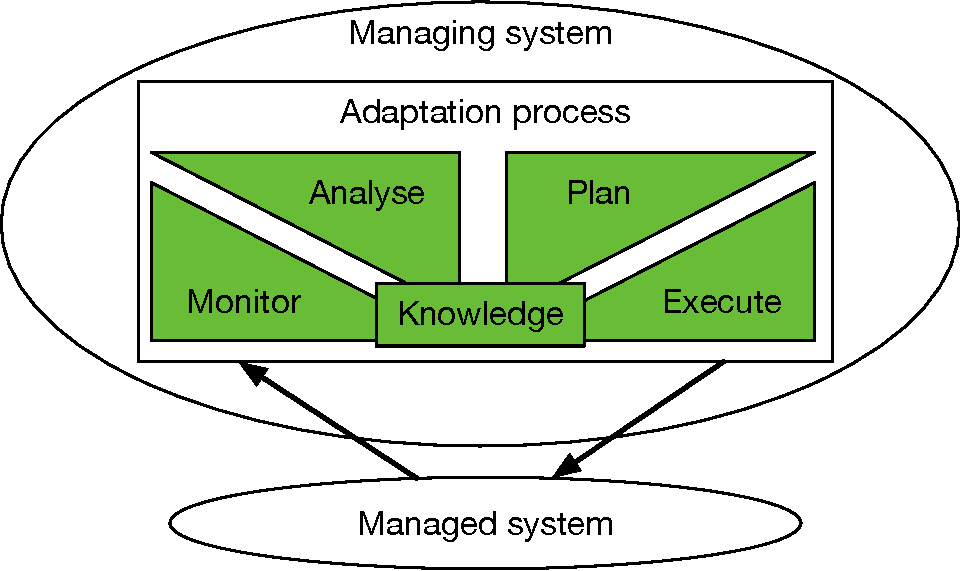
\includegraphics[width=0.6\linewidth]{img/chapt-background/adptSyst/mapek}
	\caption{MAPE-k loop (based on~\cite{DBLP:journals/computer/KephartC03})}
	\label{fig:background:adptSyst:principles:mapek}
\end{figure}

In the literature, we can find different approaches to engineer \glspl{adptSyst}~\cite{DBLP:journals/computer/GarlanCHSS04}.
Among them, the most used one took its inspiration from control theory~\cite{DBLP:conf/dagstuhl/BrunSGGKLMPS09}: the feedback control loop.
The common implementation is the \gls{mapek} loop~\cite{DBLP:journals/computer/KephartC03, computing2006architectural}, shown in~\Cref{fig:background:adptSyst:principles:mapek}.
This loop is split into four phases: monitoring, analyse, planning, and executing.
During the monitoring phase, all information of the managed system and the \gls{env} are put into the knowledge.
Based on the updated knowledge, the analyse phase detects any need for adaptation using the adaptation goals.
If any, the planning phase computes the set of actions to adjust the managing system structure or behaviour.
Finally, the executing phase completes the plan.
From the \gls{mde} community, one approach to implement such a feedback look is to use the \gls{m@rt} paradigm, explained in the next section. 



%Danny Weyns have identified six waves of engineering \glspl{adptSyst}~\cite{DBLP:books/sp/19/Weyns19}.
%First, \textit{automating tasks} that focus on the automation of repetitive and error-prone management tasks of complex systems~\cite{DBLP:journals/computer/KephartC03}.
%Second, \textit{architecture-based adaptation} that defines architecture as the basis of supporting engineering of \glspl{adptSyst}. 
%Third, \textit{\gls{m@rt}}~\cite{DBLP:journals/computer/BlairBF09, DBLP:journals/computer/MorinBJFS09} that establishes a technique to link the \gls{adptSyst} with a model with a \textquote{causal connection}.
%Four, \textit{goal-driven adaptation} that emphasised on the specification of the system requirements, exposed to uncertainties, and those for the solutions.
%Five, \textit{guarantees under uncertainties} that consider uncertainty as a cornerstone concern for \glspl{adptSyst} and that define techniques to ensure the adaptation goals and the functional correctness of the adaptation components.
%Six, \textit{control-based adaptation} that stresses the use of the control theory to benefit from a robust mathematical formalism.
%Among these six waves, this thesis is part of the third one, \gls{m@rt}, that we detail in the next section.

\subsection[Models@run.time]{\Gls{m@rt}}
\label{sec:background:sas:m@rt}
The adaptation process needs to have a deep understanding of the system and its \gls{env}.
Following the \gls{mde} methodology\footnote{\gls{mde} is a methodology that promotes the usage of \glspl{model} for software engineering activities (\cf \Cref{sec:back:mde})}, research efforts have led to the \gls{m@rt} paradigm~\cite{DBLP:journals/computer/MorinBJFS09, DBLP:journals/computer/BlairBF09}.
It stresses the use of a model layer, causally connected to the system, and used by the adaptation process.
The causal connection encompasses two features of the \gls{model}.
First, the model reflects the up-to-date state of the system (structure and behaviour) and its \gls{env}.
Second, any modification of the model triggers a modification of the system.
In this way, the \gls{model} can be used as an interface between the system and the adaptation process, as shown in~\Cref{fig:intro:context:m@rt}.
The layer can contain several models to represent different aspect of the system at runtime~\cite{DBLP:journals/computer/MorinBJFS09}: structure, \gls{behaviour}, \gls{env}, \etc{}
Moreover, it can contains representation that guide the adaptation process~\cite{DBLP:journals/computer/CetinaGFP09, DBLP:journals/computer/HallsteinsenHPS08} such as configurations point.

Following the \gls{mapek}, the model layer should structure the knowledge.
In this thesis, we define a metamodel of this knowledge to enable developers diagnosing, understanding, and reasoning over \gls{longTermAct} (\cf \Cref{chapt:tkm}).
In the next section, we thus characterise the information that composes the knowledge.


%The adaptation process needs to have a deep understanding of the system and its \gls{env}.
%Following the \gls{mde} methodology\footnote{\gls{mde} is a methodology that promotes the usage of \glspl{model} for software engineering activities (\cf \Cref{sec:back:mde})}, research efforts have led to the \gls{m@rt} paradigm~\cite{DBLP:journals/computer/MorinBJFS09, DBLP:journals/computer/BlairBF09}.
%The paradigm defines a \gls{model} that is \textquote{causally connected} to the system.
%The \gls{model} abstracts the structure and the behaviour of the system, the \gls{env}, and the adaptation goals.
%The causal connection encompasses two features of the \gls{model}.
%First, the model reflects the up-to-date state of the system (structure and behaviour) and its \gls{env}.
%Second, any modification of the model triggers a modification of the system.
%In this way, the \gls{model} can be used as an interface between the system and the adaptation process, as shown in~\Cref{fig:intro:context:m@rt}.
%
%Using this approach, we can say that engineers use a model-based architecture.
%Morin \etal described a possible solution that is characterised by three layers, four types of runtime models, and five elements~\cite{DBLP:journals/computer/MorinBJFS09}.
%The three layers are: online model space, causal connection, and business application.
%The business application layer contains the logic of the system.
%It has sensors for monitoring and actuators (here called factories).
%This layer is connected to the online model space, which is platform-independent, through the causal connection layer.
%The online model space contains the four different runtime models: feature, context, reasoning, and architecture model.
%The feature model represents the different configuration points of the system.
%The context model abstracts the relevant part of the system and the \gls{env}.
%The reasoning model links between the first two models by associating the features with a particular context.
%Finally, the architecture model specifies the different entities of the system.
%These models are exchanged by the five elements that implement the adaptation mechanism.
%First, the \textit{event processor}, which implements the monitoring stage of the \gls{mapek} loop, updates the context model with information received through the sensors.
%Second, the \textit{goal-based reasoner}, which implements the analyse phase, uses the feature and reasoning model to select the new features for adjusting the system and achieving the goals.
%Third, the \textit{model weaver}, which implements a part of the planning stage, transforms the selected features into a new architecture model, checked by the \textit{configuration checker}.
%Finally, the configuration manager, which implements a part of the planning stage and the executing one, computes and executes the sequence of actions to reach the proposed architecture model.
%
%More generally, this solution stresses the use of a model layer, causally connected to the system, and used by the adaptation process.
%Following the \gls{mapek}, the model layer should structure the knowledge.
%In this thesis, we define a metamodel of this knowledge to enable developers diagnosing, understanding, and reasoning over \gls{longTermAct} (\cf \Cref{chapt:tkm}).
%In the next section, we thus characterise the information that composes the knowledge.

\subsection{Characterisation of information of the knowledge}

\begin{table}
		\centering
    	\begin{tabular}{p{0.15\linewidth}p{0.78\linewidth}}
    		\hline
    		\textbf{Element} & \textbf{Description} \\
    		\hline
    		Context & Context data are characterised by: their volatility, their temporality, their uncertainty, their source, or their connection.\\
    		Requirement & Three kinds of requirements: performance, specific quality, and constraint. \\
    		Action & Four pieces of information characterise an action: requirement(s) to achieve, initial context, effects, and execution information (start time, end time, status).\\
    		\hline
    	\end{tabular}
    	\caption{Characterisation of information of the knowledge}
    	\label{table:background:adptSyst:charc}
\end{table}


\subsubsection{General concepts of adaptation processes}

Similar to the definition provided by Kephart~\cite{DBLP:journals/computer/KephartC03}, IBM  defines adaptive systems as \textquote{a computing environment with the ability to manage itself and \textbf{dynamically adapt} to change in accordance with \textbf{business policies and objectives}. [These systems] can perform such activities based on \textbf{situations they observe or sense in the IT environment} [...]}~\cite{computing2006architectural}.

Based on this definition, we can identify three principal concepts involved in adaptation processes.
The first concept is \textbf{actions}. 
They are executed to perform a dynamic adaptation through actuators.
The second concept is \textbf{business policies and objectives}, which is also referred to as the \textbf{system requirements} in the domain of (self-)adaptive systems.
The last concept is the observed or sensed \textbf{situation}, also known as the \textbf{context}.
The following subsections provide more details about these concepts.
\Cref{table:background:adptSyst:charc} gives an overview of these different elements.

\subsubsection{Context}

In this thesis, we use the widely accepted definition of context provided by \linebreak Dey~\cite{DBLP:journals/puc/Dey01}: \textquote{Context is \textbf{any information that can be used to characterize} the situation of an entity. An entity is a person, place, or object that is considered relevant to the interaction between a user and [the system], including the user and [the system] themselves}.
In this section, we list the characteristics of this information based on several works found in the literature~\cite{DBLP:conf/pervasive/HenricksenIR02, DBLP:conf/seke/0001FNMKT14, DBLP:journals/percom/BettiniBHINRR10, DBLP:journals/comsur/PereraZCG14}.
We use them to drive our design choices of our \textit{Knowledge} \gls{metamodel} (\cf Section~\ref{sec:tkm:mm:knoeldge}).

\paragraph{Volatility}
Data can be either \textbf{static} or \textbf{dynamic}.
Static data, also called frozen, are data that will not be modified, over time, after their creation~\cite{DBLP:conf/pervasive/HenricksenIR02, DBLP:journals/comsur/MakrisSS13, DBLP:journals/percom/BettiniBHINRR10}.
For example, the location of a machine, the first name or birth date of a user can be identified as static data. 
Dynamic data, also referred to as volatile data, are data that will be modified over time.

\paragraph{Temporality}
In dynamic data, we may be interested not only in storing the latest value, but also the previous ones~\cite{DBLP:conf/seke/0001FNMKT14, DBLP:conf/pervasive/HenricksenIR02}. 
We refer to these data as \textbf{historical} data.
Temporal data is not only about past values, but also future ones. 
Two kinds of future values can be identified, \textbf{predicted} and \textbf{planned}.  
Thanks to machine learning or statistical methods, dynamic data values can be \textbf{predicted}. 
\textbf{Planned} data are set by a system or a human to specify planned modification on the data.

\paragraph{Uncertainty}
One of the recurrent problems facing context-aware applications is the data uncertainty~\cite{DBLP:conf/dagstuhl/LemosGMSALSTVVWBBBBCDDEGGGGIKKLMMMMMNPPSSSSTWW10, DBLP:conf/pervasive/HenricksenIR02, DBLP:journals/comsur/MakrisSS13, DBLP:journals/percom/BettiniBHINRR10}.
Uncertain data are not likely to represent reality. They contain noise that makes it deviate from its real value.
This noise is mainly due to the inaccuracy and imprecision of sensors.
Another source of uncertainty is the behaviour of the environment, which can be unpredictable.
All the computations that use uncertain data are also uncertain by propagation.

\paragraph{Source}
%According to the literature, data sources are grouped into two main categories, either sensed (measured) data or computed (derived) \linebreak data~\cite{DBLP:journals/comsur/PereraZCG14}.
%We refine this with an additional category called profiled.
%Profiled data may be set either by a user (\textbf{profiled by a human}) or by an external system (\textbf{profiled by an external}).
In this dissertation, we distinguish three main categories of data source: sensed, computed, profiled, and given.
Sensed data are thous measured by a sensor (hardware of software).
Computed data result from a process that combine different data.
And profiled data are those that are learned.
Finally, given data are static data manually set in a software.

\paragraph{Connection}
Context data entities are usually linked using three kinds of connections: conceptual, computational, and consistency~\cite{DBLP:conf/pervasive/HenricksenIR02, DBLP:journals/percom/BettiniBHINRR10}.
The conceptual connection relates to  (direct) relationships between entities in the real world (e.g. smart meter and concentrator).
The computational connection is set up when the state of an entity can be linked to another one by a computation process (derived, predicted). 
Finally, the consistency connection relates to entities that should have consistent values. For instance, temperature sensors belonging to the same geographical area.

\subsubsection{Requirement}
\label{sec:back:adapt:knowledge:req}

Adaptation processes aim at modifying the system state to reach an optimal one.
All along this process, the system should respect the \textbf{system requirements} established ahead. 
Through this thesis, we use the definition provided by IEEE~\cite{iso2017systems}: ``(1) Statement that translates or expresses a need and its associated \textbf{constraints} and \textbf{conditions}, (2) \textbf{Condition or capability that must be met or possessed} by a system [...] to satisfy an agreement, standard, specification, or other formally imposed documents".\looseness=-1

Although in the literature, requirements are categorised as functional or non-func\-tional, in this document we use a more elaborate taxonomy introduced by Glinz~\cite{DBLP:conf/re/Glinz07}.
It classifies requirements in four categories: functional, performance, specific quality, and constraint.
All these categories share a common feature: they are all temporal.
During the life-cycle of an adaptive system, a stakeholder can update, add or remove some requirements~\cite{DBLP:conf/icse/ChengA07, pandey2010effective}.

\subsubsection{Action}
In the IEEE Standards~\cite{iso2017systems}, an action is defined as: \textquote{\textbf{process of transformation} that \textbf{operates upon data} or other types of inputs to create data, produce outputs, or \textbf{change the state} or condition of the subject software}.

In the context of adaptive systems, we can define an action as a process that, given the context and requirements as input, adjusts the system behaviour.
This modification will then create new data that correspond to an output context. In the remainder of this document, we refer to the output context as impacted context, or effect(s).
Whereas requirements are used to add preconditions to the actions, context information is used to drive the modifications.
Actions executions have a start time and a finish time. They can either succeed, fail, or be cancelled by an internal or external actor.

\subsection{Key concepts for this thesis}
\Glspl{adptSyst} have been proposed to tackle the growing complexity of systems (structure and behaviour) and their \gls{env}.
One common model for implementing them is the well-known \gls{mapek} loop, a feedback control loop based on shared knowledge.
Applying the \gls{m@rt} paradigm, this knowledge can be structured by a \gls{model}, which is causally connected to the system.
This \gls{model} should represent the uncertain and time dimension of the knowledge.
In this thesis, we consider that the knowledge comprises information related to the context, the actions, and the requirements.
In this thesis, we propose a \gls{metamodel}\footnote{A \gls{metamodel} is a \gls{model} that defines another \gls{model} (\cf \Cref{sec:back:mde}).} to represent the decisions made by the adaptation process over time (\cf \Cref{chapt:tkm}).
Additionnaly, we define a language, \langName, to propagate uncertainty in the computation made during the adaptation process (\cf \Cref{chapt:aintea}).







